
\documentclass[a4paper]{article}
\usepackage[left=3cm,right=3cm,top=2cm,bottom=2cm]{geometry} % page settings
\usepackage{amsmath} % provides many mathematical environments & tools
\usepackage{titlesec}
\usepackage{graphicx}
\usepackage{algorithm,caption}
\usepackage[utf8]{inputenc}
\usepackage[noend]{algpseudocode}
\graphicspath{ {images/} }
\usepackage{xparse}% http://ctan.org/pkg/xparse
\usepackage{mathtools}
\usepackage{courier}
\usepackage{verbatim}
\DeclarePairedDelimiter\ceil{\lceil}{\rceil}
\DeclarePairedDelimiter\floor{\lfloor}{\rfloor}


\setlength{\parindent}{0mm}
\titleformat{\subsection}[runin]
{\normalfont\Large\bfseries}{\thesection}{1em}{}
\titleformat{\subsubsection}[runin]
{\normalfont\large\bfseries}{\thesubsection}{1em}{}

\begin{document}
	
	\title{Secure \& Dependable Systems \\  Spring 2017 \\ Assignment 05}
	\author{Humza Abid}
	\maketitle
	
	\subsection*{Problem 5.1} \textit{Verification: Class Invariants} \\
	
	The given class invariant holds true since in the context of the program and input variables for each method, the precondition holds true, the process terminates and then the post condition holds true (the invariant in question, in this case). This can be seen easily when the object \textit{size}, a private member, is always constant throughout all the methods, ie. an increase or decrease of it is realized in every method of it. We can see further that the class invariant is \textit{strong} since the invariant would hold in its own class each time a new instance of the class is called. 
		
	\subsection*{Problem 5.2} \textit{Verification: Class Invariants} \\
	
	Choice of class: \textit{Date}.\\
	For the chosen class, the invariant is:
	\begin{verbatim}
		1 <= day && day <= 31, 1 <= month && month <= 12        
	\end{verbatim}
	
	Note, that this invariant is only a \textit{weak invariant} since it does not hold true for all class instances (esp. in the case of February).
	
	\begin{verbatim}
		fun yesterday(){
		if(month % 2 == 0){	
			if(day == 1){
			return day = 31, month - 1;
			}else{
			return day - 1, month;
			}	
		}elseif(month % 2 != 0){
			if(month == 3 && day == 1){
				return day = 28, month - 1;
			}elseif(day == 1){
			return day = 30, month - 1;}
		}else{
			day - 1, month;
		}
		}
	\end{verbatim}
	
	\pagebreak
		
	\begin{verbatim}
	fun tomorrow(){
	if(month % 2 == 0){
		if(month == 2 && day == 28){
		return day = 1, month + 1;
		}elseif(day != 30){
		return day + 1, month;
		}else{
		return day = 1, month + 1;
	}elseif(month % != 0){
		if(day != 31){
		return day + 1, month;
		}else{
		return day + 1, month + 1;
		}
	}
	\end{verbatim}	
	
	\subsection*{Problem 5.3} \textit{Verification: Pure Functions} \\
	
	\textbf{Base Case:} $zero + m \, == \, m + zero$ \\
	Applying \textit{zero\_left} and \textit{zero\_right} $\implies m \, == \,m$. \\
	\textbf{Inductive hypothesis:} $n + m\, ==\, m + n$ \\
	\textbf{Proving for succ(n):} $succ(n) + m \, == \, m + succ(n)$
	$\implies succ(n+m) \, == \, m+ succ(n)$ \\
	Using the Inductive Hypothesis: $succ(m+n) \, == m+ succ(n)$
	$\implies m+ succ(n) \, == m+ succ(n) $ \textbf{QED.}
	
	\subsection*{Problem 5.4} \textit{Proof Assistants: Practice} \\
	
	I installed Isabelle, and ran a simple function (addition for natural numbers) detailed in the notes. The screen shots details the function, and corresponding outputs:
	
	\begin{figure}[ht]
		\centering
		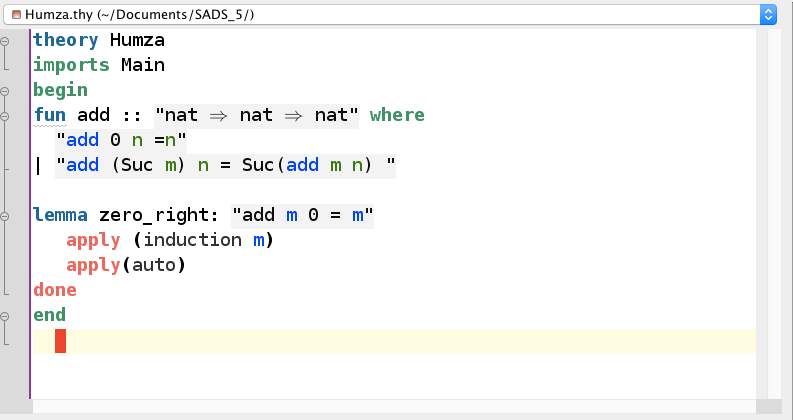
\includegraphics[width=0.7\textwidth, scale=0.7]{1.png}
		\caption*{}
		\label{1}
	\end{figure}
	
	\begin{figure}[ht]
		\centering
		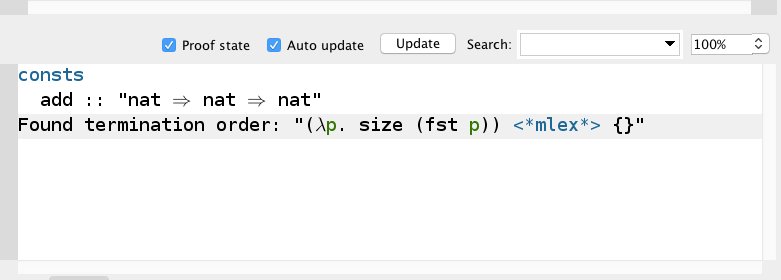
\includegraphics[width=0.7\textwidth, scale=0.7]{2.png}
		\caption*{}
		\label{2}
	\end{figure}
		
	\begin{figure}[ht]
		\centering
		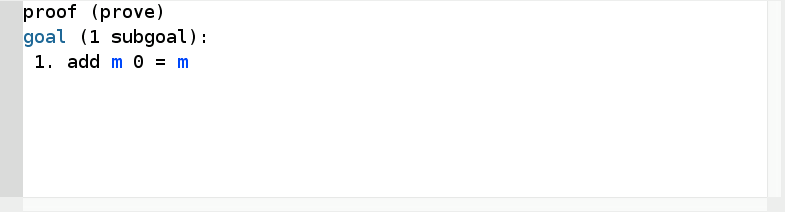
\includegraphics[width=0.7\textwidth, scale=0.7]{3.png}
		\caption*{}
		\label{3}
	\end{figure}
	
	\begin{figure}[ht]
		\centering
		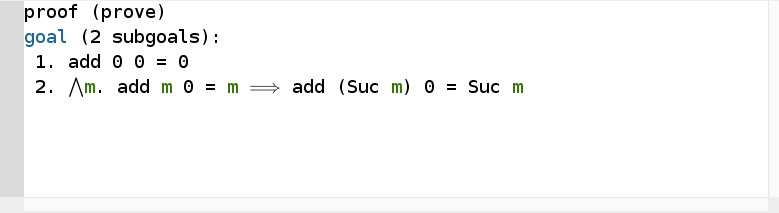
\includegraphics[width=0.7\textwidth, scale=0.7]{4.png}
		\caption*{}
		\label{4}
	\end{figure}
	
	\begin{figure}[ht]
		\centering
		
\includegraphics[width=0.7\textwidth, scale=0.7]{5.png}
		\caption*{}
		\label{5}
	\end{figure}
	
	 
\end{document}